%% ----------------ATENCIÓ-----------------------
%% Aquest document està preparat per codificació 
%% UTF-8. Si es llegeix amb un editor 
%% preparat per una altra codificació alguns 
%% caràcters no es veuran correctament.
%%---------------------------------------------- 
%%
%% Aquest document vos pot servir de base per la
%% realització de la memòria del treball final de
%% grau. Es recomana seguir els consells que 
%% apareixen en els diferents comentaris del 
%% document. Convindrà mantenir l'estructura
%% d'aquest exemple i introduir canvis sols 
%% allà on s'indiqui.
%%
%%-----------------------------------------------
%%
%% La plantilla preparada per a la realització de
%% la memòria és la classe LaTeX TFGEPSUIB.cls
%% que es fonamenta en la classe memoir. Aquesta
%% emula alguns `packages` que, per tant, no serà
%% necessari incloure dins el vostre document. El
%% manual de memoir explica quins són aquests
%% paquets (per exemple booktabs, array, tabluarx). 
%% Per altra banda, TFGEPSUIB també carrega 
%% automàticament els paquets, fontenc, xcolor, 
%% graphicx i microtype.
%%
%%-----------------------------------------
%% Opcions de la classe TFGEPSUIB:
%%
%% Per defecte, la classe TFGEPSUIB suposa
%% que la memòria es redactarà en català i que 
%% els estudis són els de Grau en Enginyeria
%% telemàtica. 
%%
%% Si preferiu utilitzar el castellà o anglés
%% per a la redacció de la memòria podeu
%% fer-ho indicant-ho a les opcions.
%\documentclass[catalan]{TFGEPSUIB}
\documentclass[english,GINF]{TFGEPSUIB}
%%
%% Per indicar quins són els estudis pels quals
%% es redacta la memòria heu d'incloure una de
%% les següents opcions:
%%
%% GTEL - Grau en Enginyeria Telemàtica
%% GMAT - Grau de Matemàtiques
%% GINF - Grau d'Enginyeria Informàtica
%% GEDI - Grau d'Enginyeria d'Edificació
%% GELE - Grau d'Eng. Elec. Ind. i Automàtica
%% GAGR - Grau en Eng. Agroali. i del Medi Rural
%%
%% Per escriure la memòria en castellà pels estudis
%% de matemàtiques, la línia inicial serà
%\documentclass[spanish,GMAT]{TFGEPSUIB}
%%------------------------------------------

% Per incloure expressions matemàtiques en
% el document és recomanable usar els paquets
%\usepackage{amsmath,mathtools} 

% Per incloure fragments de codi hi ha diferents
% paquets disponibles. Triau el que vos sigui 
% més convenient, per exemple listings. 
%\usepackage{listings} 

% Amb tcolorbox podeu definir caixes per llistats,
% teoremes, exemples, ...
%\usepackage{tcolorbox}

% Si voleu que les referències bibliogràfiques
% apareguin amb el format "autor-any" en comptes 
% de "número" heu d'usar el paquet natbib.
%\usepackage[round,colon,sort&compress]{natbib} 

% En general, la documentació tècnica pot
% incloure molts acrònims. Per això es recomana
% usar el següent paquet. Consultau el corresponent
% manual per saber com s'usa.
\usepackage[printonlyused]{acronym}

% Les diferents unitats de mesura tenen un
% format estàndard de representació que convé
% respectar. Per això s'usa el paquet `siunitx`.
% També permet representar nombres en notació
% científica i alinear correctament els valors 
% numèrics a les taules. Pegau una ullada al 
% manual. Si no voleu usar-lo comentau la línia. 
\usepackage{siunitx}

% Com que és convenient que el paquet hyperref
% sigui un dels darrers en carregar-se, si voleu 
% afegir nous paquets, feis-ho a continuació.
%\usepackage{}
\graphicspath{ {imgs/} }
\usepackage{subcaption}

% El paquet "hyperref" crea enllaços automàticament 
% dins el document. Aquests enllaços permeten la 
% navegació a través de les diferents referències 
% figures, bibliografia, fórmules, índex, ...
% tant sols assenyalant-los amb el ratolí. 
\usepackage[backref, colorlinks=true, all colors=black]{hyperref}

% Si voleu que els enllaços apareguin en colors diferents,
% eliminau l'opció "all colors=black". 

%----------------------------------------------
% Dades de la Portada amb els valors adequats
% La portada inclou informació del estudis,
% títol del projecte, autor(s) del projecte,
% tutor(s) i data. 
%
% Els estudis ja s'han definit amb la opció
% corresponent, però si el projecte
% és d'uns altres estudis no definits a les
% opcions, com són, per exemple, els dels plans
% anteriors, sempre podeu usar la comanda \estudis
% per definir-los.
% Per exemple, per l'enginyeria tècnica en 
% telemàtica podeu usar:
%\estudis{Enginyeria Tècnica en Telecomunicacions, especialitat Telemàtica}

\estudis{Degree in informatic engineering}

% Aquí podeu posar el títol de la vostra memòria
\title{Tetris Neural Net playing in the Nintendo Switch}

% Nom de l'autor del TFG.
\author{Joan Dot Sastre}

% La comanda \tutor mostra el nom del director
% a la portada interior. Si hi ha més d'un tutor
% caldrà fer un petit canvi. Demanau ajuda. 
\tutor{José María Buades Rubio \&
Gabriel Moyá Alcover}

% Indicau el curs acadèmic que correspongui.
\date{Academic Year 2020-21}

% Indicau les paraules claus del vostre treball.
\paraulesclau{AI, deep learning, deep q learning, tetris}

% Si l'autor no autoritza la publicació del treball
% descomentau la línia següent
%\autorfalse

% Si el tutor no autoritza la publicació del treball
% descomentau la línia següent
%\tutorfalse

%---------------------------------------------------------------------------------------------------------------------------------------------------------------

% Durant l'escriptura de la memòria haureu de 
% compilar-la moltes vegades. Si voleu guanyar
% una mica de temps, podeu dividir el contingut
% en diferents fitxers i compilar-ne sols alguns.
% La comanda següent és la que vos permet
% definir quins compilar i quins no.

%\includeonly{Instruccions,Annexos}

% Quan vulgueu treballar amb tot el document, 
% simplement, comentau la línia anterior.  

\begin{document}

% Recordau haver indicat, títol, autor i tutor
% i no toqueu les línies següents.
\portada
\portadainterior
\frontmatter

% Voleu dedicar i agrair el treball a algú?
% Activau les línies següents i escriu el
% que vulguis dins l'entorn 'agraiments' 
%
\cleartorecto \thispagestyle{empty}
\begin{agraiments}
Thanks to José María Buades, for suggesting such a nice idea of a final degree project and helping me throughout all the steps whenever i needed.
\end{agraiments}

% A continuació el Sumari
\cleartorecto \tableofcontents

% Si voleu que apareguin una llista de figures
% i taules, activau les línies corresponents
%\cleartorecto \listoffigures
%\cleartorecto \listoftables 

% Si apareixen molts acrònims a la documentació
% convindrà fer-ne una llista. Podeu veure com
% crear-la consultant el fitxer 'Acronims.tex',
% que és el que s'inclou aquí.
\chapter{Acrònims} %Respectau títol del capítol.
%
% Per utilitzar els acrònims es recomana fer un poc 
% de recerca bibliogràfica per entendre com 
% funcionen. Concretament podeu llegir el manual
% que teniu dins el vostre sistema.
% La comanda `texdoc acronym` hauria de mostrar-lo.
%
\begin{acronym}

\acro{AMC}[AMC]{Adaptive Modulation and Coding}

\acro{EPS}[EPS]{Escola Politècnica Superior}

\acro{IP}[IP]{Internet Protocol}

\acro{LTE}[LTE]{Long Term Evolution}

\acro{MIMO}[MIMO]{Multiple-Input Multiple-Output}

\acro{OFDM}[OFDM]{Orthogonal Frequency Division Multiplexing}

\acro{OFDMA}[OFDMA]{Orthogonal Frequency Division Multiple Access}

\acro{RDI}[R+D+I]{Recerca, Desenvolupament i Innovació}

\acro{TCP}[TCP]{Transport Control Protocol}

\acro{TDMA}[TDMA]{Time Division Multiple Access}

\acro{TFG}[TFG]{Treball Final de Grau}


\end{acronym}
 
% Si no usau acrònims, comentau la línia anterior

% En l'arxiu Resum.tex es posarà el resum
% del treball.
%!TeX root=MemoriaTFG.tex

\chapter{Resum}

La capacitat de redacció i presentació oral de treballs científics i tecnològics és una de les competències més importants per al desenvolupament personal i professional d'un científic o d'un enginyer. Per tal de millorar aquestes competències, aquest document presenta una breu introducció a les habilitats que s'han de treballar per tal de ser un bon comunicador en qualsevol de les activitats acadèmiques i professionals.

Atès que en l'àmbit universitari la normativa del \ac{TFG} ens obliga a la redacció d'una proposta i d'una memòria de \ac{TFG} i a la defensa oral d'aquest treball davant d'un tribunal, en aquest document s'utilitza el \ac{TFG} com a exemple per introduir els principis bàsics per a la redacció i presentació de treballs. Tanmateix, les recomanacions que s'hi fan són prou generals com perquè puguin ser fàcilment esteses a altres activitats de comunicació científico-tecnològica.

D'una banda, a partir de la normativa de \acsp{TFG} de l'\ac{EPS} es descriuen les diferents etapes que s'han de superar fins a la defensa oral del \ac{TFG} i de l'altra, s'intenta donar resposta a preguntes del tipus: Què és el que fa que la documentació o la presentació oral d'un treball siguin bones? Quines són les millors passes a fer per redactar una bona documentació o per preparar una bona presentació? Quina ha de ser l'estructura global de la documentació o de la presentació?  

% No toqueu la línia següent 
\mainmatter\pagestyle{ruled}

%%%%%% COS DEL TREBALL %%%%%%%%%%%%

% Una bona pràctica consisteix en dividir
% un document llarg en diferents fragments,
% per exemple per capítols, i incloure aquests
% fragments dins el fitxer principal amb la
% comanda \include. Així, podem escriure la 
% comanda \includeonly{llista fitxers a compilar}
% que ens permetrà processar sols aquella part
% del document que ens interessi.

%!TeX root=MemoriaTFG.tex

\chapter{Introduction}
\section{Artificial intelligence in video games}

AI has been present in video games since the very beginning.
Its purpose has always been to improve the players experience and the methods that have been used to implement such behaviours are vast, ranging from finite state machines and increasingly more complex enemy movement patterns tied to the game difficulty/level, to combining different advanced methods like pathfinding and decision trees. Other techniques related to machine learning such as reinforcement learning can currently also be found in some games. All these methods are mostly used for \ac{NPC}s and the information they perceive from the environment can be given in two different ways, via sensors, which provide a limited vision of the game world, or via the game’s own stored information e.g., the player’s exact location.

Due to an increasing interest in artificial intelligence in recent years, people have started to try and beat their favourite games with it. When taking this approach, we must first consider how the agent is going to perceive the game, having the same two options we talked about before. This time we usually encounter a major inconvenience, we do not have direct access to the game information due to us not being the game developers, although thanks to some \ac{API}(such as OpenAI Gym) we can access the game and thus base our agent’s information on it. Unfortunately, those APIs mostly feature older games, which limits us to the ones provided by it. Hence comes the need for image processing tools to extract data, though this may not necessarily be done by us, as will be shown later.

Due to the increasingly more difficult games being beaten, has also come a need for more intricate agents, leading to the drop of simpler techniques in favour of reinforcement learning (many times paired with those old techniques in order to provide the agent with basic behavioural guidance). This has ended up providing much better results than previously achieved in highly complex environments, and also helped discover new strategies in the own game. Even exploits in the system have sometimes been found, like in the case of an OpenAi project, where in a hide and seek game, the agents managed to abuse the physics engine in various ways. 

%\hypertarget{openai}{openai}

\section{Objectives and setbacks}

The overall goal of the project has already been discussed, but what will be called a success has not yet been defined.
Building an AI capable of playing Tetris has already been done many times before with great success, although the challenge trying to be taken on has a few more major and minor hindrances.

First of all, as a minor inconvenience, the Tetris version we are building our AI on features the \ac{SRS}, which is a modern rotation system with some unconventional situational rotations. No implementation that can be used has been found, neither as an OpenAI gym nor as simple game. Because of this, an entire game replicating Tetris 99 must be built from scratch to train our model.

Secondly, there is not a standardized way to access the console’s controller port from a PC, so a reliable workaround must be built and adapted. This is probably the biggest setback.

Lastly, and as a result of having to intercommunicate both devices, some extra delay, that we hope will not heavily interfere, will occur when bringing everything together.

Having mentioned the setbacks we first encounter, we expect to build an agent that plays tetris to near perfection, never loosing a game and trying to make as many points as possible in the least amount of time. If anything, we expect only the conditions outside the agents power to make it perform badly, namely bad screen detections or missed inputs. This means that once a good enough agent has been built, our main focus will shift onto making it perform as closely as possible to its intended actions on the console. 

\section{Task division}

In order to reach our goal, we have to tackle the problems one by one. Thus, the means by which the results in the project have been obtained consist of dividing it into four different modules:
\begin{itemize}
	\item	Switch-PC interface: The way in which the pc is able to communicate with the console.

\item	Information capture: How the console’s information is sent to the pc and then processed for use by the neural net.

\item	Machine learning: How the AI is able to learn. Includes the training environment explanation, the heuristic used and how it was chosen.

\item	Decision making: Defines how the information extracted by the information capture module is treated right before it is finally ready to be sent to the net. It also explains how the output is adapted and transferred to the console correctly.
\end{itemize}

The aforementioned modules will be further explained later, in their corresponding section in the document but, it needs to be mentiones that the whole project has been made in python given its many machine learning library options.









%!TeX root=MemoriaTFG.tex

\chapter{Tetris 99 and system built}

\section{Tetris version}
Tetris is a long running game series that has been ongoing since 1984, when Alexey Pajitnov invented it. Ever since it was created, many iterations of the game have been made, with each one of those somewhat altering the rules or adding new mechanics to spice things up. As previously mentioned, the project is being made under the Tetris 99 version, which implements the \ac{SRS}. This version has been chosen due to it being the most modern tetris up to date and because of the challenge of having our \ac{AI} work on another platform. 

\section{Game basics}
\begin{figure}[]
\centering
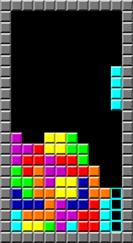
\includegraphics{image001}
\caption{\label{fig:gridExample}Tetris grid example}
\end{figure}

\begin{figure}[]
\centering
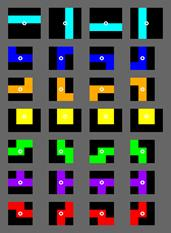
\includegraphics{image002}
\caption{\label{fig:pieces}Tetris pieces and their rotations}
\end{figure}

\begin{table}[h]
\begin{tabular}{
>{\columncolor[HTML]{F8F9FA}}l 
>{\columncolor[HTML]{F8F9FA}}l lll}
Single             & 100 × level difficulty   \\
Double             & 300 × level difficulty   \\
Triple             & 500 × level difficulty   \\
Tetris (Quadruple) & 800 × level difficulty 
\end{tabular}
\caption{\label{fig:scores}Tetris score by lines cleared}
\end{table}

\begin{table}[]
\begin{tabular}{
>{\columncolor[HTML]{F8F9FA}}l 
>{\columncolor[HTML]{F8F9FA}}l }
\hline
Combo       & 50 ×   combo count × level \\
Soft drop   & 1 per   cell               \\
Hard   drop & 2 per   cell              
\end{tabular}
\caption{\label{fig:scores2}Tetris score by movement and combos}
\end{table}

As many people already know, Tetris is a puzzle game consisting in trying to stack pieces up pieces and clear lines on a 10x20 grid. Whenever a line is filled to its maximum capacity it gets cleared and the blocks above it drop as many lines as were cleared. Whenever a piece is locked in place in an altitude higher than the game grid plus one you lose. A grid could look like figure~\ref{fig:gridExample}.

There is a total of 7 different pieces, each one of those having an associated colour that is usually maintained through all Tetris versions. Their names are I, J, L O, S, T and Z as seen in figure ~\ref{fig:pieces}.

As we can see in the image just referenced, each piece has four different orientations which can be accessed sequentially back and forth in the order shown, the small circle indicating the axis the piece rotates in.

The I and O pieces are a special case given that they do not use an actual block as their anchor point to rotate, making the first one shift one block up or down depending on the current position and the second one not rotate at all.

Now that we know their shapes, we see that the maximum number of lines that can be cleared at once is four. This is crucial because the score we obtain does not increase linearly, netting us higher scores the more lines we clear in one go.

The actual formula which dictates how many points we get can be seen in ~\ref{fig:scores}

More ways of obtaining points are soft drops (moving the piece down one cell), hard drops (letting the piece fall to the bottom) and combos (chaining line clears with different pieces), which go as \ref{fig:scores2}

Finally, there is T-spins, which is a mechanic that will be spoken about at the end of this block, once all the information surrounding the SRS has been laid out.
The scoring system just described works on single player game modes, but in Tetris 99, the main game mode actually involves 99 players concurrently battling against each other. Here line clears serve another purpose, sending “garbage lines” to the opponents. More on this system in the following section.


\section{UI and specifics}
\begin{figure}[]
\centering
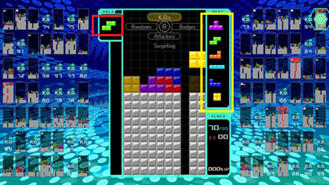
\includegraphics{image003}
\caption{\label{fig:tetris99game}Actual Tetris 99 game}
\end{figure}

An actual game of Tetris 99 will look like fig\ref{fig:tetris99game}.
There are many things that need to be analyzed to fully understand all the game aspects of this game version.

The first thing that should be mentioned is that we can see the upcoming 6 pieces that will have to be placed on the board (highlighted by the yellow square). Those are chosen from a bag containing all seven pieces, therefore making the game much more predictable as luck will not be impacting the game as much as with a fully random selector.

Then, there is the piece storage block (encapsulated by the red square), which allows us to save the current piece and draw the next one or, if there already is a stored one, to swap it out.

Last and more importantly, the background shows many more smaller Tetris boards, which belong to other players who are competing against you. In this mode you cannot see your score, and your performance is based on surviving the longest. When clearing lines, you now send garbage lines (grey blocks) to whoever of those players you are targeting:
\begin{itemize}
	\item	Clear two lines: Send one line of garbage
	\item	Clear three lines: Send two lines of garbage
	\item	Clear four lines: Send four lines of garbage
	\item	Clear the full board: +4 lines of garbage
\end{itemize}

Whenever you kill a player, a part of a badge is awarded to you. Each badge is increasingly more difficult to get, and you can only get up to four in total:
\begin{itemize}
   \item	Two knockouts: 25\% garbage bonus
   \item	Six knockouts:   50\% garbage bonus
   \item	14 knockouts:    75\% garbage bonus
   \item	30 knockouts:    100\% garbage bonus
\end{itemize}

It may seem quite difficult to complete all badges, but the method is eased by being able to steal the badges from a player you have defeated.
You can choose between five attacking modes to target different opponents:
\begin{itemize}
   \item	K.O.s: targets whoever is closer to losing the game.
   \item	Randoms.
   \item	Badges: targets whoever has more badges.
   \item	Attackers: targets whoever is attacking you.
   \item	Choice: manually select a specific player.
\end{itemize}

If you are targeted by multiple opponents, a boost to attack power is received:
\begin{itemize}
   \item	2 Opponents:	+1 Bonus lines sent
   \item	3 Opponents:	+3 Bonus lines sent
   \item	4 Opponents:	+5 Bonus lines sent
   \item	5 Opponents:	+7 Bonus lines sent
   \item	6+ Opponents:	+9 Bonus lines sent
\end{itemize}

This boost is applied before the badge attack boost.

It should also be noted that when receiving garbage lines, those will first be shown in the column right under your piece storage, and only be added to your board after some time. The time is indicated by 3 colour stages, being grey, yellow, and red, from best to worst. Garbage lines can also be cleared before they are added to your board by simply clearing lines.

\section{SRS (Standard rotation system)}
Now we can focus on the most intricate part of the game, the rotation system. The basics of this system have already been mentioned, however there is a much deeper pattern to it, which allows us to rotate pieces into places we would not normally be able to. These situations occur when a rotation that is not possible because a collision is detected, and the system tries to move the piece into four different offsets sequentially, sticking to whichever one works first. There are mainly two kinds of offsets, the ones that straight up ignore some collisions and allow you to rotate passing through blocks, and the ones that move you to another location. When an offset displaces you, it is known in game terms as a “kick”, and it should be noted that kicks can be performed against walls and pieces equally, propelling you in on or even two directions at the same time, even upwards. Because of the existence of upward kicks, a system limiting the number that can be performed had to be implemented to avoid infinite stalling.

As there is a very large variety of rotations and kicks that can be performed, only a few examples that represent most cases can be seen in figures \ref{fig:phase1}, \ref{fig:phase2}, \ref{fig:phase3}, \ref{fig:phase4}.

\begin{figure}
\centering
\begin{subfigure}{.4\textwidth}
  \centering
  
\includegraphics[width=.6\linewidth]{image004}
\end{subfigure}%
$\rightarrow$
\begin{subfigure}{.4\textwidth}
  \centering
  
\includegraphics[width=.6\linewidth]{image005}
\end{subfigure}
\caption{\label{fig:phase1}No kick phase}
\end{figure}

\begin{figure}
\centering
\begin{subfigure}{.3\textwidth}
  \centering
  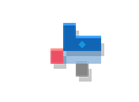
\includegraphics[width=.8\linewidth]{image006}
\end{subfigure}%
$\rightarrow$
\begin{subfigure}{.3\textwidth}
  \centering
  
\includegraphics[width=.8\linewidth]{image007}
\end{subfigure}%
$\rightarrow$
\begin{subfigure}{.3\textwidth}
  \centering
  
\includegraphics[width=.8\linewidth]{image008}
\end{subfigure}
\caption{\label{fig:phase2}Right kick phase}
\end{figure}

\begin{figure}
\centering
\begin{subfigure}{.3\textwidth}
  \centering
  
\includegraphics[width=.8\linewidth]{image009}
\end{subfigure}%
$\rightarrow$
\begin{subfigure}{.3\textwidth}
  \centering
  
\includegraphics[width=.8\linewidth]{image010}
\end{subfigure}%
$\rightarrow$
\begin{subfigure}{.3\textwidth}
  \centering
  
\includegraphics[width=.8\linewidth]{image011}
\end{subfigure}
\caption{\label{fig:phase3}Up right kick phase}
\end{figure}

\begin{figure}
\centering
\begin{subfigure}{.4\textwidth}
  \centering
  
\includegraphics[width=.6\linewidth]{image012}
\end{subfigure}%
$\rightarrow$
\begin{subfigure}{.4\textwidth}
  \centering
  
\includegraphics[width=.6\linewidth]{image013}
\end{subfigure}
\caption{\label{fig:phase4}Down kick phase}
\end{figure}

Now that we have showed some examples, we can talk about T-spins. As its own name implies T-spins are performed using the T piece, and they happen whenever we manage to offset the piece into clearing 1, 2 or three lines, giving us 2, 4 and 6 garbage lines/800 × level, 1200 × level, 1600 × level respectively.

\begin{figure}[h]
\centering
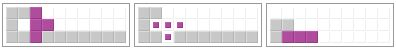
\includegraphics{image014}
\caption{\label{fig:tspin1}T-spin single}
\end{figure}

\begin{figure}
\centering
\begin{subfigure}{.33\textwidth}
  \centering
  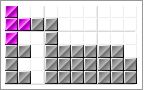
\includegraphics[width=.8\linewidth]{image015}
\end{subfigure}%
\begin{subfigure}{.33\textwidth}
  \centering
  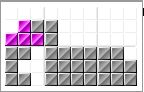
\includegraphics[width=.8\linewidth]{image016}
\end{subfigure}%
\begin{subfigure}{.33\textwidth}
  \centering
  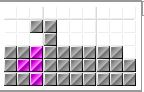
\includegraphics[width=.8\linewidth]{image017}
\end{subfigure}
\caption{\label{fig:tspin2}T-spin double}
\end{figure}

\begin{figure}[h]
\centering
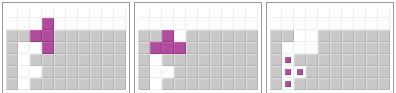
\includegraphics{image018}
\caption{\label{fig:tspin3}T-spin triple}
\end{figure}


\section{Our system}
Having defined all important aspects of tetris 99, an environment similar enough had to be built in order for the \ac{AI} not to find itself in a foreign situation when being tested in the Nintendo Switch. Thus a search for similar looking tetris implementations had to be done. Unfortunately, as mentioned when talking about the project setbacks, no complete candidates where found.

Thanks to the information found regarding how the \ac{SRS} works and a project giving an example implementation in C\#, we built from scratch a similar looking system that fulfilled our requirements. The system is constituted by three classes, board, piece and tile, each one being controlled and used by the one mentioned before it. Finally, the the script called "tetris.py" unites all of them together and creates a visual interface to play on and show the net's output whenever requested.

To explain the following data structure a bottom up approach will be used in order to follow the thought process behind its implementation.

\subsection{Tile}
Tile is a class very short class containing a position in two dimensions (x,y) and a colour in rgb format. It also includes a method that given a center point and a direction, rotates its own coordinates once.

\subsection{Piece}
A piece object is consituted by "n" number of tiles depending on the piece type. There is a piece child class for each possible piece type and every one of them contains a list of each of the displacements or kicks that can be performed given a rotation. The method rotate piece loops through each tile calling their own rotate method using the center tile as the anchor.

\subsection{Board}
Board is the biggest class of the three consituting the data structure. It is in charge of implementing all the tetris 99 rules there are. Here there is also a piece rotating method, which is in charge of checking wether a kick can be performed or not, given it has the position of each of the blocks and the walls. Despite having implemented the t-spin moves a system that puntuates them has not been built, as it will not be used to reward the neural net (more information on that in the neural net section). 

\subsection{Tetris game}
Finally, we have the tetris script, coded using pygame. There is two different implementations within it which will be used to our convenience. The first one calls the main game loop and allows us to play the game normally, reading our keyboard input and calling the appropiate board methods to perfrom each one of them:

\begin{itemize}
   \item	$\downarrow$: "Soft drop", drops the piece down by one line.
   \item	$\uparrow$: "Hard drop", drop the piece as far down as it can.
   \item	$\leftarrow$: Moves left by one column if possible.
   \item	$\rightarrow$: Moves right by one column if possible. 
   \item	space bar: Stores the current piece if a piece was not just stored.
   \item	"a": Rotates left.
   \item	"d": Rotates right.
\end{itemize}

The second one is used by the neural net to show each of its moves. This means that the board game object is manipulated solely by the AI and the scrpit is only used to render the visual information of it by calling the applicable methods.

Either way, both can be stopped by exiting the window clicking the top right "X".

% !TEX root=MemoriaTFG.tex

\chapter{Switch-PC interface}
A key aspect to the project consist in how we connect the \ac{PC} and the console. The first part of it, getting the images from the game, has already been dealt with in the previous chapter, but now comes the challenging part. We need to somehow make the neural net's output get to the console.

\section{Approaches and final solution}
As mentioned in the introduction, there is no way to control the Nintendo switch besides using its own controller. The first thing that came to mind was building a robot capable of pressing the buttons itself whenever we told it to. A rough way of implementing it was thought about and some actual piece candidates where found, but nothing came of it, as the difficulty of building such device could be a final project of its own.

Parallely, a way of faking the pc as a controller was investigated. A project that could record input onto an arduino and then send it to the switch by connecting it directly into the console's controller port, was found, which told us that accessing the console was possible. This works by using the same checking protocol sequence as a Nintendo controller when trying to connect the device.

By modifying the project, we allowed for it to instead of record some input sequence, receive it from the PC. As the project comes with a python script that contains the whole controller scheme and methods to test and ensure a good connection, we can plug the script directly in our project for its future use.

\section{Arduino tools}
The original project only used the arduino seen in image \ref{arduino}, which already had the commands imprinted in a loop. This time around, as it is connected to our \ac{PC} using a USB-TTL converter (\ref{appendix:USBTOTTL}), seen in \ref{USBtoTTL}, the loop waits for the input and sends it to the console.

The USB-TTL converter must be connected according to the information given by the own device, which means that contrary to what is most common, RX to TX and TX to RX, it is done backwards. This is only because the converter tells us where the connection must go and not what it actually is. As for the ground and 5V cables there is no room for doubt.

\begin{figure}[h]
\centering
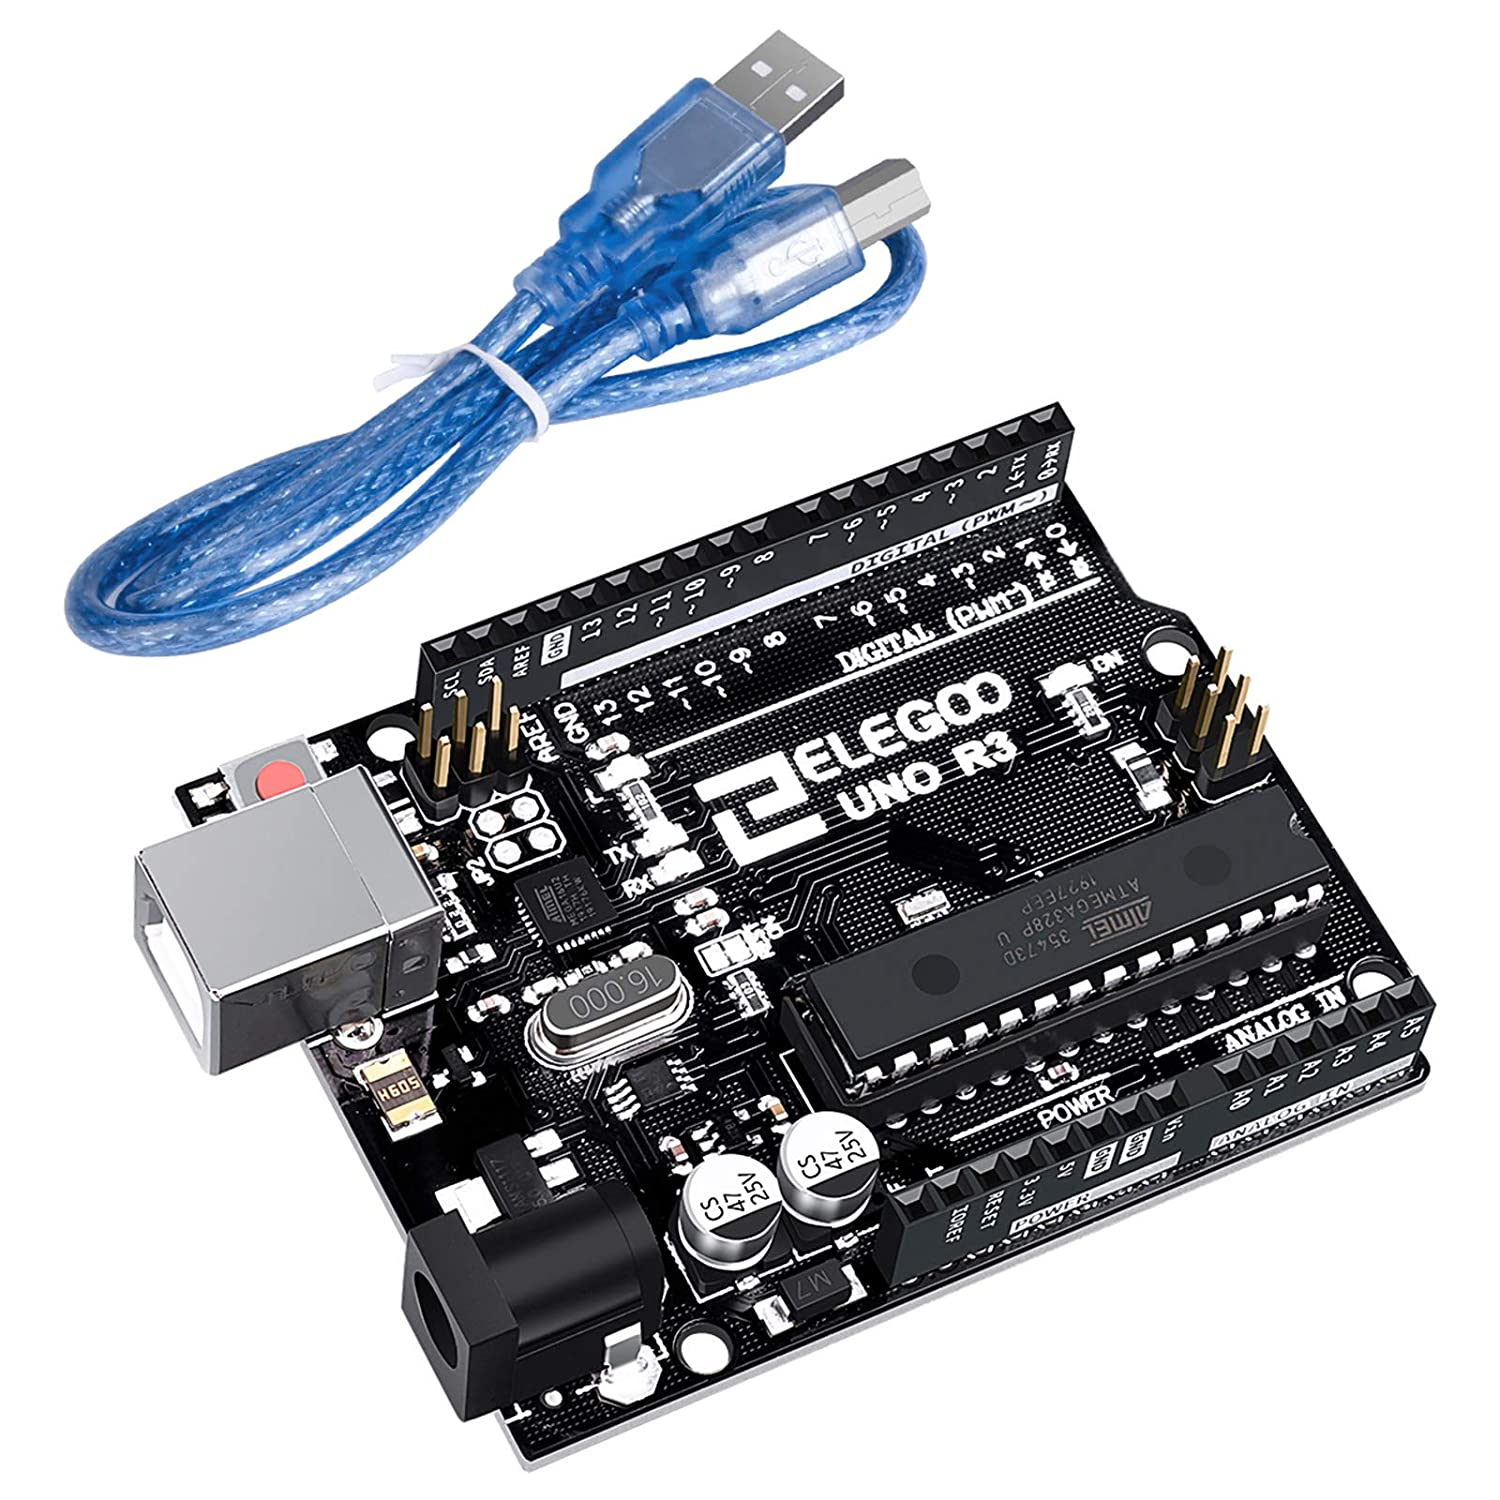
\includegraphics[width=.4\linewidth]{image024}
\caption{\label{arduino}Arduino ELEGOO UNO R3}
\end{figure}
\begin{figure}[h]

\centering
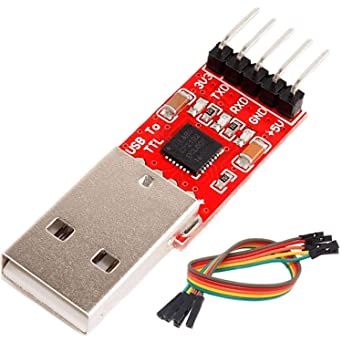
\includegraphics[width=.4\linewidth]{image025}
\caption{\label{USBtoTTL}USB to TTL CP2102}
\end{figure}
% !TEX root=ManualTFG.tex

\chapter{Information capture}
If we want to play on the Switch, a system that allows us to decrypt what is on screen, to feed it to the neural net is needed. Our first approach was to use some sort of video device, like a webcam, to record what was on screen while simultaneously sending that information to the \ac{PC}. That idea was quickly scrapped, as using a normal capture card was the obvious easiest go to. Thanks to that, we can use Opencv (see more in \ref{appendix:opencv}) to get the images directly in real time with minimal delay in order to perform whichever operations we need to. OpenCV was chosen as our image processing tool mainly because of its vast number of examples and information regarding it.

\section{Detection}
As previously mentioned, a game of Tetris 99 looks like the image in \ref{fig:highlighted}:
 
\begin{figure}[h]
\centering
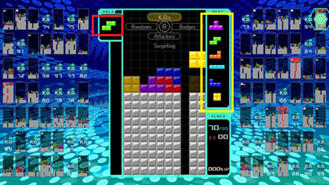
\includegraphics{image003}
\caption{\label{fig:highlighted}Highlighted detection areas}
\end{figure}

Given that the most important information we need is what are the pieces currently in play, a method to detect whether there is one and which type it is had to be devised. At first it was thought this could be guessed by the piece’s own shape but, given rotations and having access to the colour channel, a detection by the later method was much faster and easier to do. Thus, came the idea of calculating the mean colour of each shape in a $5\times 5$ matrix from its center point, including empty blocks and grey pieces. Still, as seen in the previous image, when a piece is placed, it turns a darker tone of its former colour, making us have to factor those in. Thanks to this minor inconvenience, we will later be able to distinguish the main piece from an already placed one if we need to do so. Finally, a small leeway to the mean colour of each piece had to be taken into account when checking for matches due to other elements in the game board influencing the colour of the own piece with shines or shades.

The information we get is also presented back to the user in real time by drawing the conclusions on top of the processed frame. This helps us understand what is being detected and therefore being fed to the neural net. Depending on the detection a string matching the detection will be shown:

\begin{itemize}
	\item	"e": Means empty block.
	\item	"S", "Z", "I", "T", "J", "L", "O": Refers to each of the possible pieces found in a tetris game.
	\item	"gr": Means grey block.
\end{itemize}

There is one more element that will not be shown as a letter, "No match", which will be displayed using the last letter found in the block in white, otherwise their respective piece colour or black for the empty will be shown.

\subsection{Game grid}
The first element we try to detect is the game grid. It can be done thanks to having manually found where the cells center pixel is, and how wide and tall each cell is. By applying a for loop, we can then iterate through each cell and store the information in two arrays with the size of the game grid ($10\times 20$). The first array contains 0's for empty cells, 1's for blocks and 2's for the main piece (game\_matrix), while the second one contains information related to the  colour, including a “no match” variable (info\_matrix). On each iteration, game\_matrix block will be updated only if a match was found, else it will assume the board’s state has not changed.

\subsection{Out of the grid}
The next element we detect is a line upwards out of the main game matrix (row 21). This must be done due to the main piece spawn position going up when it cannot be placed at a certain height, the maximum being 21. This was done separately due to the background colour not being black and because only the main piece is displayed at that height, with placed blocks being hidden by the borders \ref{mainout}, \ref{blocksout}.

%\subsubsection{Main piece out of grid}
\begin{figure}[h]
\centering
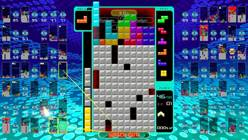
\includegraphics{image020}
\caption{\label{mainout}Main piece out of grid}
\end{figure}

%\subsubsection{Blocks out of grid}
\begin{figure}[h]
\centering
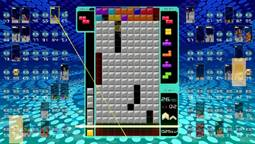
\includegraphics{image021}
\caption{\label{blocksout}Blocks out of grid}
\end{figure}

\subsection{Check stored piece}
To detect which piece (or if none) is in storage, a system that casts two rows of three detection points was built. Each one of those points corresponds to a possible place of a block and, in case it is filled, it updates two matrices with the same system that was built for the game grid detection.

\subsection{Check upcoming pieces}
In order to know what is coming up next, we reused the system to detect stored pieces, this time iterating through a for loop once for each of the upcoming six pieces. Each of the matrices detected is then stored in an array in the same order they are detected (top to bottom).

\section{How noise affects detection}
As mentioned before, we cannot differentiate piece colours without adding a small margin of error for the detection to be consistent in the majority of cases. Unfortunately not only are the colours influenced by other elements, but also visual effects spawn all across the game board depending on the actions done.

To begin with, there is an effect that tells us where our piece is going to be placed (see figure \ref{effects}). Luckily this feature was found to be able to be turned off in the game options, although it is the only one that can be filtered out this easily.

As for the other effects, things like red screen borders, arrows pointing other players and glitter when dropping a piece or sending grey blocks to opponents can also be found interfering with detections (some also seen in \ref{effects}). Many of those directly block what is behind them, so no image processing or margin can be set to minimize or eliminate the obstruction. The best solution we came across is not updating the board information whenever a foreign object is detected, which ends up working pretty well as many of the effects disappear pretty quickly.

\begin{figure}[h]
\centering
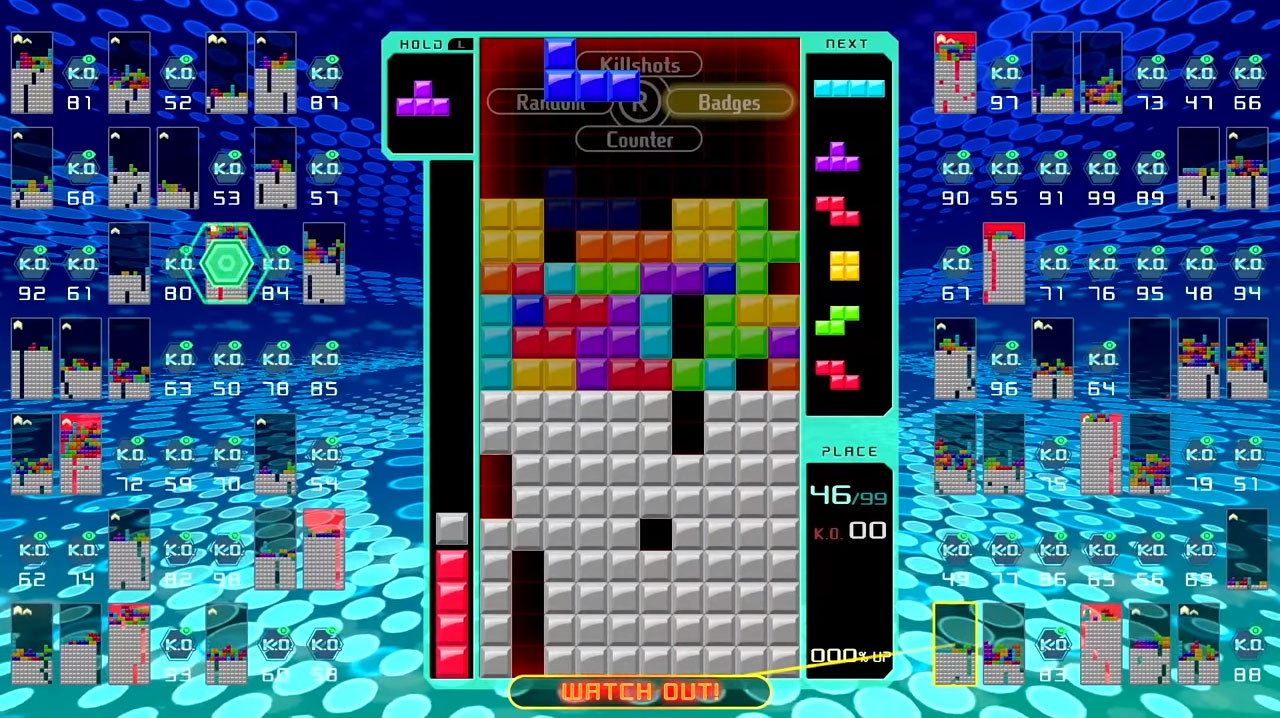
\includegraphics[width=.8\linewidth]{image023}
\caption{\label{effects}Game effects}
\end{figure}

\section{Information adaptation for the neural net}
Once all the information needed has been collected, a way of adapting it so that the neural net understands it had to be made. To do so, we had to convert the data into a Board object of our own Tetris game, with the same configuration detected.

As our neural net works by finding the best combination of consecutive rotations and horizontal movement, and then dropping the piece, we only need to ask for the neural net’s response once (when the piece just spawned). This way we only try to detect new information when the last sequence of movements is completed and when a new piece is detected at the top five rows of the grid, which are the only rows a piece can spawn in plus two more, in case there is a late detection.

When a new main piece is detected, which as mentioned before can be done thanks to it being able to be told apart from the rest because of being slightly brighter, we construct a Piece object with its type and position. The type can easily be guessed by just checking the first blocks's colour but the position is trickier. As all pieces always spawn in the same exact rotation and x position, we can always assign it to be the same, "4", as for the height, we it will be the one of the first block found -1, given that each piece's center block is always one row down except for the "I" piece.

We can now proceed with the creation of the game grid that will be added to the Board object. It is quite simple to do so given that we have a $10\times 20$ array stored with information regarding each cell. We now only have to filter out the main piece, add four empty rows at the top and reverse it to match the object’s model. The actual colour of the placed blocks does not matter, as it is merely an aesthetic element.

Finally, we check if there is a stored piece. If positive, we must then check its colour to know if it is an option for it to be placed or not. That information is then passed on to the Board object.


% !TEX root=MemoriaTFG.tex

\chapter{Deep learning module}\label{deep learning}

Here
%!TeX root=MemoriaTFG.tex

\chapter{Decision making}

To make the code cleaner, a separated module called FileVideoStream, that takes care of handling the frames was used

%!TeX root=MemoriaTFG.tex

\chapter{Results}

Having performed 
%!TeX root=MemoriaTFG.tex

\chapter{Conclusion}


%%%%%%% Fi cos del treball %%%%%%%%%%%

% Si el vostre document no conté apèndixs 
% comentau les dues línies següents
\appendix 
%!TeX root=MemoriaTFG.tex

\chapter{Format final}

\section{Paper i impressió}

\subsection{Paper}

Cal utilitzar paper mida DIN A4 vertical (210 x 297 mm), el qual, a més de ser l'estàndard més generalitzat, és el format predeterminat de
la majoria de processadors de textos. No es recomana que el cos del TFG tengui una extensió superior a les 80 cares. Si la longitud del
treball és superior, s'hauria de pensar en passar informació cap als annexos.

\subsection{Impressió a dues cares}

La presentació del document ha de ser a dues cares a partir de la introducció i fins al final del document. Fixau-vos que la plantilla
\LaTeX\ ja produeix un document adequat per a la seva impressió a doble cara.

\section{Enquadernació}

Cal realitzar l'enquadernació amb espiral negra. Les tapes superior i inferior seran de plàstic transparent i negre, respectivament.

\section{La plantilla de \LaTeX}

La plantilla de \LaTeX\ d'aquest document defineix els marges, la tipografia, estils i espaiat de tots els elements per la memòria del treball de final de
grau. Una vegada es compila el document, \LaTeX\  adequarà el text al format definit en la plantilla. A més, \LaTeX\ realitzarà de forma
automàtica tot un seguit de funcions que us facilitaran la feina amb la memòria, com per exemple: numerar els capítols, seccions, i
sub-seccions; inserir els encapçalaments i números de pàgina; crear de forma automàtica els índexs de continguts, figures i taules \dots
Per tant, l'usuari només es preocuparà del text que està introduint, no serà necessari pensar en cap moment en l'aspecte final del
document. Serà \LaTeX\ qui aplicarà el format de la plantilla al teu text.

Aquesta plantilla està fonamentada en la classe \texttt{memoir}. Això presenta l'avantatge de que com que aquest format inclou automàticament altres \emph{packages}, per exemple \texttt{booktabs},
\texttt{array}, \texttt{tabularx}, etc., no caldrà carregar-los en el preàmbul del vostre document. Això també significa que totes les comandes de \texttt{memoir} estan a la vostra disposició per editar la memòria, per tant, és molt recomanable consultar el seu manual~\cite{Wil10}.

Amb el format de plantilla que s'ha definit només s'enumeraran 3 nivells de profunditat, a part dels capítols. Per definir-los s'utilitzaran les
següents expressions de \LaTeX:

\begin{verbatim}
\chapter{Nom del capítol}
\section{Nom de la secció}
\subsection{Nom de la sub-secció}
\subsubsection{Nom de la sub-sub-secció}
\end{verbatim}

\section{Fórmules, figures i taules}
\subsection{Fórmules}

El format de les fórmules es troba definit en la plantilla i \LaTeX\ l'aplica cada vegada que es compila el document.

Per escriure fórmules en \LaTeX\ s'hauran d'utilitzar les expressions adients. Aquí es presenta un exemple de codi:
\begin{verbatim}
\begin{equation}\label{NomEq}
\zeta= m \sum _{i=0}^{N} \left( \frac{\beta}{\sigma _i \lambda_ j}
\right)^{2} \cos (2\pi f_i)
\end{equation}
\end{verbatim}
que produeix el següent resultat:
\begin{equation}\label{NomEq}
\zeta= m \sum _{i=0}^{N} \left( \frac{\beta}{\sigma _i \lambda_ j}\right)^{2} \cos (2\pi f_i).
\end{equation}

Citar l'expressió anterior és tant senzill com fer:
\begin{verbatim}
L'equació \ref{NomEq} determina $\ldots$
\end{verbatim}
L'equació \ref{NomEq} determina $\ldots$

\subsection{Figures}

A continuació es mostra el codi \LaTeX\ per incloure una figura continguda en un fitxer.

\begin{verbatim}
\begin{figure}
\begin{center}

\includegraphics[width=0.2\textwidth]{./LogoUIB.jpg}
\caption{Exemple de figura}
\label{NomFig}
\end{center}
\end{figure}
\end{verbatim}
El resultat es pot veure a la Fig.~\ref{NomFig}.

\begin{figure}
\begin{center}

\includegraphics[width=0.2\textwidth]{./LogoUIB.jpg}
\caption{Exemple de figura}
\label{NomFig}
\end{center}
\end{figure}

Es pot modificar la variable \texttt{width} per ajustar l'amplada de la figura com més ens convingui. Teniu en compte que la variable
\texttt{\textbackslash textwidth} guarda el valor de l'amplada del text dins la pàgina i, per tant, és una bona referència per delimitar amplades de figura. Així doncs, la figura \ref{NomFig} ocupa la meitat de l'amplada del text en una pàgina. El format final de la figura està definit per la
plantilla i \LaTeX\ s'encarrega de presentar-la de forma convenient.

\subsection{Taules}

Les taules definides en \LaTeX\ s'enumeren automàticament i el format segueix les definicions especificades en la plantilla.

Seguidament, a mode d'exemple, es presenta el codi \LaTeX\ necessari per crear
la taula \ref{NomTaula} que apareix més avall:
\begin{verbatim}
\begin{tabular}{@{}llS@{}} 
\toprule
\multicolumn{2}{c}{Cotxes} \\ 
\cmidrule(r){1-2}
{Posició} & {Descripció} & {Velocitat màxima}\\
 & &  \multicolumn{1}{c}{(\unit{\kilo\meter\per\second})} \\ 
\midrule
1 & Vermell & 120 \\
2 & Blau & 80.1 \\
3 & Verd & 92.50 \\
4 & Blanc & 33.33 \\
5 & Negre & 56.3 \\ 
\bottomrule
\end{tabular}
\caption{Exemple de taula} \label{NomTaula}
\end{table}
\end{verbatim}
\begin{table}
\centering
\begin{tabular}{@{}llS@{}} \toprule
\multicolumn{2}{c}{\textbf{Cotxes}} \\ 
\cmidrule(r){1-2}
{\textbf{Posició}} & {\textbf{Descripció}} & {\textbf{Velocitat màxima}}\\
 & &  \multicolumn{1}{c}{(\unit{\kilo\meter\per\second})} \\ 
\midrule
1 & Vermell & 120 \\
2 & Blau & 80.1 \\
3 & Verd & 92.50 \\
4 & Blanc & 33.33 \\
5 & Negre & 56.3 \\ \bottomrule
\end{tabular}
\caption{Exemple de taula} \label{NomTaula}
\end{table}

L'entorn \texttt{tabular} que ofereix \LaTeX\  és molt complet i permet crear
multitud de taules diferents, tot i que alhora és bastant complexe. No són les
intencions del present document descriure la sintaxis i el format d'aquest
tipus d'entorn. Es poden trobar molt fàcilment \emph{tutorials} o altres informacions
per aprendre a utilitzar de forma adient aquesta sintaxis o qualsevol altra de
\LaTeX. És bastant recomanable llegir la documentació del \emph{package}
\texttt{booktabs}\footnote{No cal incloure la comanda  \texttt{\textbackslash usepackage\{booktabs\}} dins el document perquè la classe ja ho fa.}~\cite{Fea05} on s'introdueixen una sèrie de comandes per a poder realitzar
taules de més qualitat com la de l'exemple, també es defineixen quines han de
ser les pautes per fer una taula d'aspecte formal. En aquest exemple concret també s'han usat les columnes \texttt{S} i \texttt{s} que ofereix el paquet \texttt{siunitx}~\cite{Wri12}. Un efecte similar es podria aconseguir amb les columnes de tipus \texttt{D} que inclou \texttt{memoir}~\cite[Cap. 11]{Wil10}.

Cal fixar-se en que \LaTeX\ insereix les figures i taules sempre al principi de pàgina. Per tant, no cal preocupar-se per la seva posició
dintre del document s'insereixen sempre en la mateixa posició de forma automàtica.

\section{Bibliografia}

A la bibliografia s'han de llistar conjuntament llibres i articles de revistes.
Citar una referència bibliogràfica és tant fàcil com fer:
\begin{verbatim}
\cite{bib1}, \cite{bib2}, \cite{bib3}
\end{verbatim}
per citar la referència \cite{bib1}, \cite{bib2}, \cite{bib3}. 

El format de la bibliografia es genera automàticament.

\section{Acrònims}

Per exemple, un acrònim ben conegut és l'\ac{IP}.
% Aquesta sentencia ens permetrà generar una entrada a la llista d'acrònims.
% En la llista d'acrònims es definiran cada un dels acronims i mitjançant l'expressió anterior podrem referenciar-los.
 

% En aquest cas sols hi ha un fitxer d'annexos,
% però podeu afegir tants \include com calgui. 

%%%%%%% Fi apèndix 

% No toqueu la línia següent 
\backmatter

% La comanda següent defineix l'estil bibliogràfic
\bibliographystyle{IEEEtran}

% La comanda següent defineix el fitxer que
% conté les referències bibliogràfiques.
% En aquest cas és el fitxer Bibliografia.bib
%\bibliography{Bibliografia} 

\end{document}